% This is "sig-alternate.tex" V2.1 April 2013
% This file should be compiled with V2.5 of "sig-alternate.cls" May 2012
%
% This example file demonstrates the use of the 'sig-alternate.cls'
% V2.5 LaTeX2e document class file. It is for those submitting
% articles to ACM Conference Proceedings WHO DO NOT WISH TO
% STRICTLY ADHERE TO THE SIGS (PUBS-BOARD-ENDORSED) STYLE.
% The 'sig-alternate.cls' file will produce a similar-looking,
% albeit, 'tighter' paper resulting in, invariably, fewer pages.
%
% ----------------------------------------------------------------------------------------------------------------
% This .tex file (and associated .cls V2.5) produces:
%       1) The Permission Statement
%       2) The Conference (location) Info information
%       3) The Copyright Line with ACM data
%       4) NO page numbers
%
% as against the acm_proc_article-sp.cls file which
% DOES NOT produce 1) thru' 3) above.
%
% Using 'sig-alternate.cls' you have control, however, from within
% the source .tex file, over both the CopyrightYear
% (defaulted to 200X) and the ACM Copyright Data
% (defaulted to X-XXXXX-XX-X/XX/XX).
% e.g.
% \CopyrightYear{2007} will cause 2007 to appear in the copyright line.
% \crdata{0-12345-67-8/90/12} will cause 0-12345-67-8/90/12 to appear in the copyright line.
%
% ---------------------------------------------------------------------------------------------------------------
% This .tex source is an example which *does* use
% the .bib file (from which the .bbl file % is produced).
% REMEMBER HOWEVER: After having produced the .bbl file,
% and prior to final submission, you *NEED* to 'insert'
% your .bbl file into your source .tex file so as to provide
% ONE 'self-contained' source file.
%
% ================= IF YOU HAVE QUESTIONS =======================
% Questions regarding the SIGS styles, SIGS policies and
% procedures, Conferences etc. should be sent to
% Adrienne Griscti (griscti@acm.org)
%
% Technical questions _only_ to
% Gerald Murray (murray@hq.acm.org)
% ===============================================================
%
% For tracking purposes - this is V2.0 - May 2012

\documentclass{sig-alternate-05-2015}


\begin{document}

% Copyright
\setcopyright{acmcopyright}
%\setcopyright{acmlicensed}
%\setcopyright{rightsretained}
%\setcopyright{usgov}
%\setcopyright{usgovmixed}
%\setcopyright{cagov}
%\setcopyright{cagovmixed}


%%% % DOI
%%% \doi{10.475/123_4}

%%% % ISBN
%%% \isbn{123-4567-24-567/08/06}

%Conference
\conferenceinfo{HPCSYSPROS '16}{November 14, 2016, Salt Lake City, UT, USA}

%%% \acmPrice{\$15.00}

%
% --- Author Metadata here ---
%%% \conferenceinfo{WOODSTOCK}{'97 El Paso, Texas USA}
%\CopyrightYear{2007} % Allows default copyright year (20XX) to be over-ridden - IF NEED BE.
%\crdata{0-12345-67-8/90/01}  % Allows default copyright data (0-89791-88-6/97/05) to be over-ridden - IF NEED BE.
% --- End of Author Metadata ---

\title{Cluster Computing with OpenHPC}
%%% \title{Alternate {\ttlit ACM} SIG Proceedings Paper in LaTeX
%%% Format\titlenote{(Produces the permission block, and
%%% copyright information). For use with
%%% SIG-ALTERNATE.CLS. Supported by ACM.}}
%%% \subtitle{[Extended Abstract]
%%% \titlenote{A full version of this paper is available as
%%% \textit{Author's Guide to Preparing ACM SIG Proceedings Using
%%% \LaTeX$2_\epsilon$\ and BibTeX} at
%%% \texttt{www.acm.org/eaddress.htm}}}
%
% You need the command \numberofauthors to handle the 'placement
% and alignment' of the authors beneath the title.
%
% For aesthetic reasons, we recommend 'three authors at a time'
% i.e. three 'name/affiliation blocks' be placed beneath the title.
%
% NOTE: You are NOT restricted in how many 'rows' of
% "name/affiliations" may appear. We just ask that you restrict
% the number of 'columns' to three.
%
% Because of the available 'opening page real-estate'
% we ask you to refrain from putting more than six authors
% (two rows with three columns) beneath the article title.
% More than six makes the first-page appear very cluttered indeed.
%
% Use the \alignauthor commands to handle the names
% and affiliations for an 'aesthetic maximum' of six authors.
% Add names, affiliations, addresses for
% the seventh etc. author(s) as the argument for the
% \additionalauthors command.
% These 'additional authors' will be output/set for you
% without further effort on your part as the last section in
% the body of your article BEFORE References or any Appendices.

\numberofauthors{2} %  in this sample file, there are a *total*
% of EIGHT authors. SIX appear on the 'first-page' (for formatting
% reasons) and the remaining two appear in the \additionalauthors section.
%
\author{
% You can go ahead and credit any number of authors here,
% e.g. one 'row of three' or two rows (consisting of one row of three
% and a second row of one, two or three).
%
% The command \alignauthor (no curly braces needed) should
% precede each author name, affiliation/snail-mail address and
% e-mail address. Additionally, tag each line of
% affiliation/address with \affaddr, and tag the
% e-mail address with \email.
  %
% TODO: update all the authors at the end....
% 1st. author
%%%\alignauthor
%%%Karl Schulz\\
%%%       \affaddr{Intel Corp.}\\
%%%       \email{karl.w.schulz@intel.com}
%%%% 2nd. author
%%%\alignauthor
%%%Reese Baird\\
%%%       \affaddr{Intel Corp.}\\
%%%       \email{reese.baird@intel.com}
}

\maketitle
\begin{abstract}
OpenHPC is a newly formed, community-based project
%Linux Foundation collaborative Project whose
that is providing an integrated collection of HPC-centric software
components that can be used to implement a full-featured reference HPC compute
resource. Components span the entire HPC software ecosystem including
provisioning and system administration tools, resource management, I/O
services, development tools, numerical libraries, and performance analysis
tools.

Common clustering tools and scientific libraries are distributed as pre-built
and validated binaries and are meant to seamlessly layer on top of existing
Linux distributions. The architecture of OpenHPC is intentionally modular to
allow end users to pick and choose from the provided components, as well as to
foster a community of open contribution. This paper presents an overview of the
underlying community vision, governance structure, packaging conventions, build
and release infrastructure and validation methodologies.

\end{abstract}



%
% The code below should be generated by the tool at
% http://dl.acm.org/ccs.cfm
% Please copy and paste the code instead of the example below. 
%
\begin{CCSXML}
<ccs2012>
<concept>
<concept_id>10010147.10010169</concept_id>
<concept_desc>Computing methodologies~Parallel computing
methodologies</concept_desc>
<concept_significance>500</concept_significance>
</concept>
<concept>
<concept_id>10002944.10011122.10002947</concept_id>
<concept_desc>General and reference~General conference
proceedings</concept_desc>
<concept_significance>300</concept_significance>
</concept>
<concept>
<concept_id>10011007.10010940</concept_id>
<concept_desc>Software and its engineering~Software organization and properties</concept_desc>
<concept_significance>300</concept_significance>
</concept>
</ccs2012>
\end{CCSXML}

\ccsdesc[500]{Computing methodologies~Parallel computing methodologies}
\ccsdesc[300]{General and reference~General conference proceedings}
\ccsdesc[300]{Software and its engineering~Software organization and properties}


%
% End generated code
%

%
%  Use this command to print the description
%
\printccsdesc

% We no longer use \terms command
%\terms{Theory}

%%% \keywords{ACM proceedings; \LaTeX; text tagging}

\section{Introduction}
Launched initially in November 2015, and formalized as a collaborative Linux
Foundation~\cite{LinuxFoundation_url} project in June 2016, OpenHPC is a
community driven project currently comprised of over 25 member organizations
from academia, research labs, and industry. To date, the OpenHPC software stack
aggregates over 60 components ranging from administrative tools like bare-metal
provisioning and resource management to end-user development libraries that
span a range of scientific/numerical uses. OpenHPC adopts a familiar package
repository delivery model and provides customizable recipes for installing and
configuring reference designs of compute clusters.

\section{Community building blocks for HPC systems}

\subsection{Motivation}
Many HPC sites spend considerable effort aggregating a large suite of 
open-source projects to provide a capable HPC environment for their users.
It is necessary to build and deploy HPC focused packages that are either absent
or outdated in Linux distro providers. Further, local packaging or 
customization frequently tries to give software versioning access to users (e.g.
via environment modules or similar equivalent). OpenHPC is focused on 
lowering the barrier to entry for HPC by providing a collection of 
pre-packaged and validated binary components that can be used to install 
and manage HPC clusters throughout their life cycle. We also provide multiple 
system configuration recipes that leverage community reference designs and best 
practices.

OpenHPC's mission is to {\em provide a reference collection of open source HPC
software components and best practices, lowering barriers to deployment,
advancement, and use of modern HPC methods and tools}.

OpenHPC components and best practices will enable and accelerate innovation and
discoveries by broadening access to state-of-the-art, open source HPC methods
and tools in a consistent environment, supported by a collaborative, worldwide
community of HPC users, developers, administrators, and vendors.



\subsection{Governance \& Community}
Under the auspices of the Linux Foundation, OpenHPC has established a governing
board and a technical steering committee. The governing board is responsible for
budgetary oversight, intellectual property policies, marketing, and long-term
road map guidance. The technical steering committee is made up of representatives
from academia, industry, and government R\&D laboratories, and is tasked with
stack architecture, component selection, releases, and day-to-day project
maintenance.

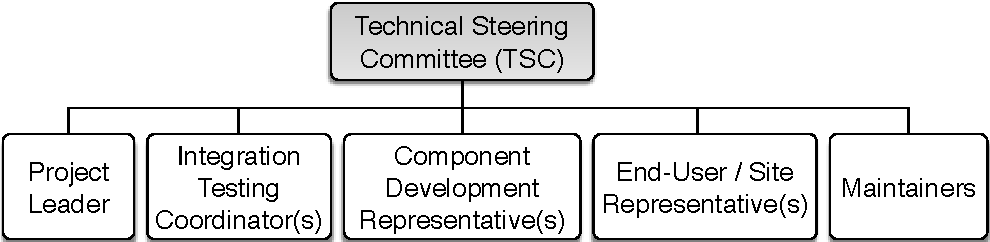
\includegraphics[width=1.0\linewidth]{figures/governance}

\subsection{Conventions}
\subsubsection{Architecture}
We have assembled a variety of common ingredients required to deploy and manage 
an HPC Linux cluster including provisioning tools, resource management, I/O 
libraries, development tools, and a variety of scientific libraries. The 
delivery mechanism is via standard package managers (i.e., there are public 
OpenHPC repositories for both yum and zypper). OpenHPC currently supports CentOS
7 and SUSE's SLE 12. A single RPM spec file generates packages for both base
operating systems. This multiple target model also extends to compiler
toolchains and MPI runtime libraries. For some components that means a spec file
can generate 12 different versions of a package. This complexity is masked by
yum/zypper convenience groups, macros within the build system, and hierarchical 
Lmod environment modules for users.

Convenience groups are prefixed with the 'ohpc-' tag, and package names have a
similar suffix. This allows for easy wild-carding with package managers, and
provides the ability to install OpenHPC-provided versions of software packages
along side of CentOS or SLE versions of the same packages.

--example showing convenience group installation, package name convention, module
load--

 - repo layout description

\subsubsection{Build}

 - spec file conventions
 - git + OBS
 
\subsubsection{Test}
 To facilitate global efforts in diagnostics/validation, we have devised a standalone integration test infrastructure
 • Intent was to create families of tests that could be used during:
 - initial install process (can we build a system?)
 - post-install process (does it work?)
 - developing tests that touch all of the major components (can we compile against 3rd party libraries, will they execute under resource manager, etc)
 • Expectation is that each new component included will need corresponding integration test collateral
 • These integration tests are included in GitHub repo


\section{Conclusions \& Future work}
Some known big ticket items on the horizon for the TSC
- establishing a process and prioritization/selection process for including
new software components
- establish minimum integration test expectations
- establish packaging conventions:
• naming schemes
• dependency hierarchy management • installation paths
• upgrade/rollback? mechanisms
- road map time line for next release (and cadence strategy for future releases)
- addition of public CI infrastructure, roll out of additional architecture builds

%ACKNOWLEDGMENTS are optional
%\section{Acknowledgments}

\bibliographystyle{abbrv}
\bibliography{hpcsyspros}


\subsection{References}
Generated by bibtex from your ~.bib file.  Run latex,
then bibtex, then latex twice (to resolve references)
to create the ~.bbl file.  Insert that ~.bbl file into
the .tex source file and comment out
the command \texttt{{\char'134}thebibliography}.
\end{document}
